\section*{3 Upper bounding the measure for a depth four circuit}
Let $\mathtt C=\sum_{i=1}^sT_i$ be a depth four circuit computing the polynomial $f=f_n$ (recall $\deg_{\mathbf x}(f_n)=d_x=\Theta(\sqrt m/\ln m)$ from Section1.1); $T_i=\prod_{j=1}^{a_i}Q_{ij}^{e_j}$ and $Q_{ij}$'s are distinct sparse polynomials computed by the $+$-gates in the third layer of $\mathtt C$, and $e_j\ge1$. We assume that $\mathbb F$ is algebraically closed and argue in Section5 why this holds without loss of generality. For brevity, we would use the terminologies 'product terms', 'sparse polynomials' and 'monomials' for the $\times$-gates, $+$-gates and $\times$-gates in the second, third and fourth layers of $\mathtt C$ respectively as shown in Figure1a. The proof of the upper bound is divided into three steps:
\paragraph{Step1:Restricting the bottom support}
In this step, we show that if $\mathtt C$ has fewer than $\Omega(m^2d_x/(\ln m)^5)$ distinct monomials then we can remove all monomials with support more than $\tau=\lfloor20\ln m\rfloor$ at a cost of setting $m$ many $\mathbf x$ variables and $m$ many $\mathbf y$ variables to zero. (Notice that if there are more than $\Omega(m^2d_x/(\ln m)^5)$ many monomials then there is nothing to prove.) This step is required not only to remove heavy gates in Step2 but also in Step3 where using the fact that all monomials have support at most $\tau$ and multilinear projection, we will argue that the degree of all monomials is not too large. More details about this restriction are given in Section3.2.1.
\paragraph{Step2:Removing heavy gates}
The transformed circuit $\mathtt C_1$, obtained after Step1, computes a polynomial in the remaining $2m$ many $\mathbf x$ variables and $2m$ many $\mathbf y$ variables. Moreover, the number of gates and the fan-in of all gates in $\mathtt C_1$ is upper bounded by the number of gates and the fan-in of the corresponding gates in $\mathtt C$. A product term in $\mathtt C_1$ is called a heavy gate if at least $w=\lfloor md_x/(\lambda_0(\ln m)^3)\rfloor$ ($\lambda_0$ is a large enough constant fixed in AppendixC) many distinct sparse polynomials are connected to it. If there are more than $m$ heavy gates, we are done. Otherwise, we remove all heavy gates using the following greedy procedure:While there is a heavy gate, evaluate a sparse polynomial that would kill the most number of heavy gates at the cost of evaluating as few monomials as possible. As we have already restricted the support of all monomials to $\tau$, we are able to argue in Section3.2.2 that this can be done at a cost of setting $m$ many $\mathbf x$ and $m$ many $\mathbf y$ variables to field constants.
These steps transform $\mathtt C$ to a 'pruned circuit', defined as follows and depicted in Figure1b.
\begin{authorclaim}{Definition6}
We say that a depth four circuit $\mathtt D$ is a pruned circuit if the support of all monomials in $\mathtt D$ is at most $\tau=\lfloor20\ln m\rfloor$, and it does not contain any heavy gate;i.e. the number of distinct sparse polynomials feeding into any product term in $\mathtt D$ is less than $w=\lfloor md_x/(\lambda_0(\ln m)^3)\rfloor$.
\end{authorclaim}
\begin{center}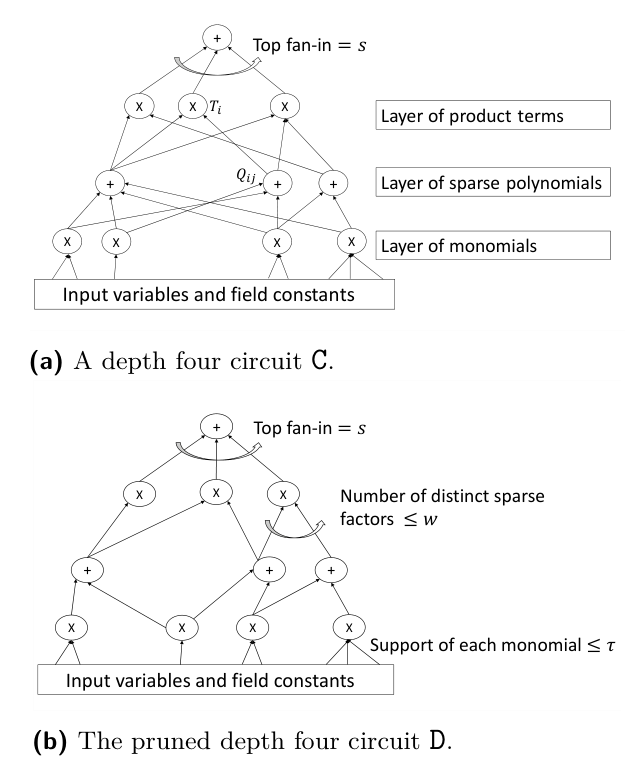
\includegraphics[width=.62\linewidth]{formal-depth4-pruning.png}\\
Figure1:A depth four circuit and its pruned version.\end{center}
\paragraph{Step3:Analysing the measure}
In this step, we analyse the measure $\PSP_{M,k,\ell}$ of the pruned circuit $\mathtt D$, obtained after Steps1 and2, computing a polynomial in the remaining $m$ many $\mathbf x$ and $m$ many $\mathbf y$ variables. More details on this analysis are provided in the following section.
\subsection*{3.1 Upper bound on the measure of a pruned depth four circuit}
Recall the definition of the measure $\PSP_{M,k,\ell}$ from Section2. In Steps1 and2, we will ensure that if a variable $x_i$ is set to a field constant then $y_i$ is also set to a field constant and vice versa. The set $M$ is then the set of indices of the remaining $\mathbf x$ (or $\mathbf y$) variables and $|M|=m$.
\begin{authorclaim}{Lemma7}
Let $\mathtt D$ be a pruned depth four circuit with top fan-in $s$ computing a polynomial in $\mathbf x_M$ and $\mathbf y_M$ variables, where $M\subseteq[3m]$, $|M|=m$. Also, let $d_x,\tau,w$ be as defined earlier, $t=\lfloor d_x/(\ln m)^3\rfloor$, $\delta=1/(\ln m)^2$, $k=\lfloor\delta d_x/t\rfloor$ and $\ell=\lfloor m/(m^{\delta/t}+1)\rfloor$. Then, for sufficiently large $m$,
\[
\PSP_{M,k,\ell}(\mathtt D)\le s\cdot m^{O(1)}\binom m{\ell+2kt\tau}\binom{\lceil w/t\rceil+k-1}{k}.
\]
\end{authorclaim}
We prove the lemma at the end of this section. As $\mathtt D=T_1+\cdots+T_s$, where $T_i$ is a product term and as $\PSP_{M,k,\ell}$ is sub-additive, to prove the lemma it suffices to show that for all $i\in[s]$,
$\PSP_{M,k,\ell}(T_i)\le m^{O(1)}\binom m{\ell+2kt\tau}\binom{\lceil w/t\rceil+k-1}{k}$.
Consider any such product term $T=\prod_{i\in[a]}Q_i^{e_i}$, where $Q_i\in\mathbb F[\mathbf x_M,\mathbf y_M]$, and since $\mathtt D$ is a pruned depth four circuit, $a\le w$. Write $Q_i=Q'_i+Q''_i$, where $Q'_i$ is the sum of all monomials of $Q_i$ wherein the individual degree of every $\mathbf x$ variable is at most two and $Q''_i=Q_i-Q'_i$. Then,
\[
T=\prod_{i\in[a]}(Q'_i+Q''_i)^{e_i}=\prod_{i\in[a]}(Q'_i)^{e_i}+Q'',
\]
where $Q''$ is a polynomial whose every monomial has a $\mathbf x$ variable with degree at least three. Thus, $\PSP_{M,k,\ell}(Q'')=0$ and hence from the sub-additivity of $\PSP_{M,k,\ell}$ we have that
$\PSP_{M,k,\ell}(T)\le\PSP_{M,k,\ell}(\prod_{i\in[a]}(Q'_i)^{e_i})$.
Let $T'=\prod_{i\in[a]}(Q'_i)^{e_i}$. We will now upper bound $\PSP_{M,k,\ell}(T')$. First, we assume without loss of generality that $a=w$ since if $a<w$ then we can multiply with additional sparse polynomials all of which are1. Next we divide the sparse polynomials into disjoint sets such that each set (except perhaps the last) has size exactly $t$. Then, we have that
\[
T'=P_1\cdots P_{\lceil w/t\rceil},\quad\text{where }P_i=\prod_{j=(i-1)t+1}^{\min(it,w)}(Q'_j)^{e_j}.
\]
\begin{authorclaim}{Claim8}
Let $P=(Q'_1)^{e_1}\cdots(Q'_t)^{e_t}$ be one of the polynomials $P_i$. For $k\ge0$, let $P^{(k)}:=\prod_{i\in[t]}(Q'_i)^{\max(e_i-k,0)}$. Then,
$\partial_{\mathbf x}^kP\subseteq\mathbb F\text{-span}\{\mathbf y_M^{\le\infty}\mathbf x_M^{\le k(2t\tau-1)}P^{(k)}\}$.
\end{authorclaim}
The proof of the claim is straighforward and is given in AppendixB.1.
\begin{proof}[Proof of Lemma7]
Recall that it is enough to show the following
\[
\PSP_{M,k,\ell}(T')\le m^{O(1)}\binom m{\ell+2kt\tau}\binom{\lceil w/t\rceil+k-1}{k},
\]
where $T'=P_1\cdots P_{\lceil w/t\rceil}$. Let $v=\lceil w/t\rceil$. Now,
\begin{align*}
\partial_{\mathbf x}^kT'
&\subseteq\mathbb F\text{-span}\{\partial_{\mathbf x}^{k_1}P_1\cdots\partial_{\mathbf x}^{k_v}P_v:k_1+\cdots+k_v=k\}\\
&\subseteq\mathbb F\text{-span}\{\mathbf y_M^{\le\infty}\mathbf x_M^{\le k_1(2t\tau-1)}P_1^{(k_1)}
\cdots\mathbf y_M^{\le\infty}\mathbf x_M^{\le k_v(2t\tau-1)}P_v^{(k_v)}:k_1+\cdots+k_v=k\}\\
&\subseteq\mathbb F\text{-span}\{\mathbf y_M^{\le\infty}\mathbf x_M^{\le k(2t\tau-1)}P_1^{(k_1)}\cdots P_v^{(k_v)}:k_1+\cdots+k_v=k\},
\end{align*}
where the second to last inclusion follows from Claim8. Hence,
\[
\mathbf x_M^\ell\partial_{\mathbf x}^kT'
\subseteq\mathbb F\text{-span}\{\mathbf y_M^{\le\infty}\mathbf x_M^{\le\ell+k(2t\tau-1)}P_1^{(k_1)}\cdots P_v^{(k_v)}:k_1+\cdots+k_v=k\}.
\]
In other words, the space of shifted partials of $T'$ is contained in the $\mathbb F$-span of polynomials of the form $Y\cdot X\cdot P_1^{(k_1)}\cdots P_v^{(k_v)}$ where $Y$ is a monomial in $\mathbf y_M$ variables and $X$ is a monomial in $\mathbf x_M$ variables of degree at most $\ell+k(2t\tau-1)$. Let us analyse the effect of the operations $\sigma_{\mathbf y_M=1}$, $[\cdot]_m$ and $\pi_{\mathbf x}$ on one such polynomial. We will assume that $\deg_{\mathbf y}(Y)\le m$ and $X$ is multilinear for otherwise the polynomial will vanish after the operations are applied. Then, we have that,
\[
\sigma_{\mathbf y_M=1}([\pi_{\mathbf x}(Y\cdot X\cdot P_1^{(k_1)}\cdots P_v^{(k_v)})]_m)
=X\cdot\sigma_{\mathbf y_M=1}([\pi_{\mathbf x}(\sigma_{\operatorname{Supp}(X)=0}(P_1^{(k_1)}\cdots P_v^{(k_v)}))]_{m-\deg(Y)}).
\]
Thus,
\begin{align*}
&\sigma_{\mathbf y_M=1}([\pi_{\mathbf x}(\mathbf x_M^\ell\partial_{\mathbf x}^kT')]_m)\\
&\quad\subseteq\mathbb F\text{-span}\{X\cdot\sigma_{\mathbf y_M=1}([\pi_{\mathbf x}(\sigma_{\operatorname{Supp}(X)=0}(P_1^{(k_1)}\cdots P_v^{(k_v)}))]_i):\\
&\qquad X\text{ is a multilinear monomial in }\mathbf x_M\text{ variables, }\deg(X)\text{ is}\\
&\qquad\text{at most }\ell+k(2t\tau-1),\quad0\le i\le m\text{ and }k_1+\cdots+k_v=k\}.
\end{align*}
Once we fix $i,X$, and $k_1,\ldots,k_v$, $X\cdot\sigma_{\mathbf y_M=1}([\pi_{\mathbf x}(\sigma_{\operatorname{Supp}(X)=0}(P_1^{(k_1)}\cdots P_v^{(k_v)}))]_i)$ is fixed. So,
\begin{align*}
\PSP_{M,k,\ell}(T')
&=\dim\left\langle\sigma_{\mathbf y_M=1}([\pi_{\mathbf x}(\mathbf x_M^\ell\partial_{\mathbf x}^kT')]_m)\right\rangle\\
&\le(m+1)\sum_{j=0}^{\ell+k(2t\tau-1)}\binom mj\binom{v+k-1}k\\
&\le(m+1)(\ell+2kt\tau)\binom m{\ell+2kt\tau}\binom{v+k-1}k\\
&=m^{O(1)}\binom m{\ell+2kt\tau}\binom{\lceil w/t\rceil+k-1}k,
\end{align*}
where the second last inequality follows from Claim9 (proved in AppendixB.1).
\end{proof}
\begin{authorclaim}{Claim9}
Let $\ell,k,t$ and $\tau$ be as defined earlier. Then, $\ell+2kt\tau<m/2$.
\end{authorclaim}
